\section{Introduction}


i want to cite \cite{fully_semi_paper_sturm}
and also \cite{vol_bary_constraint_paper} and also \cite{lecture_notes_sturm} and also \cite{nearly_conformal_paper}, 
A figure example and a text where I refer to figure \ref{shape_opt_plot} below! Additionally I need other citations like \cite{lecture_notes_faustmann_numPDE}
as well as \cite{lecture_notes_faustmann_AMF} and \cite{lecture_notes_melenk_numcomp}
yes yes yes or no?
\begin{figure}[ht]
    \centering
    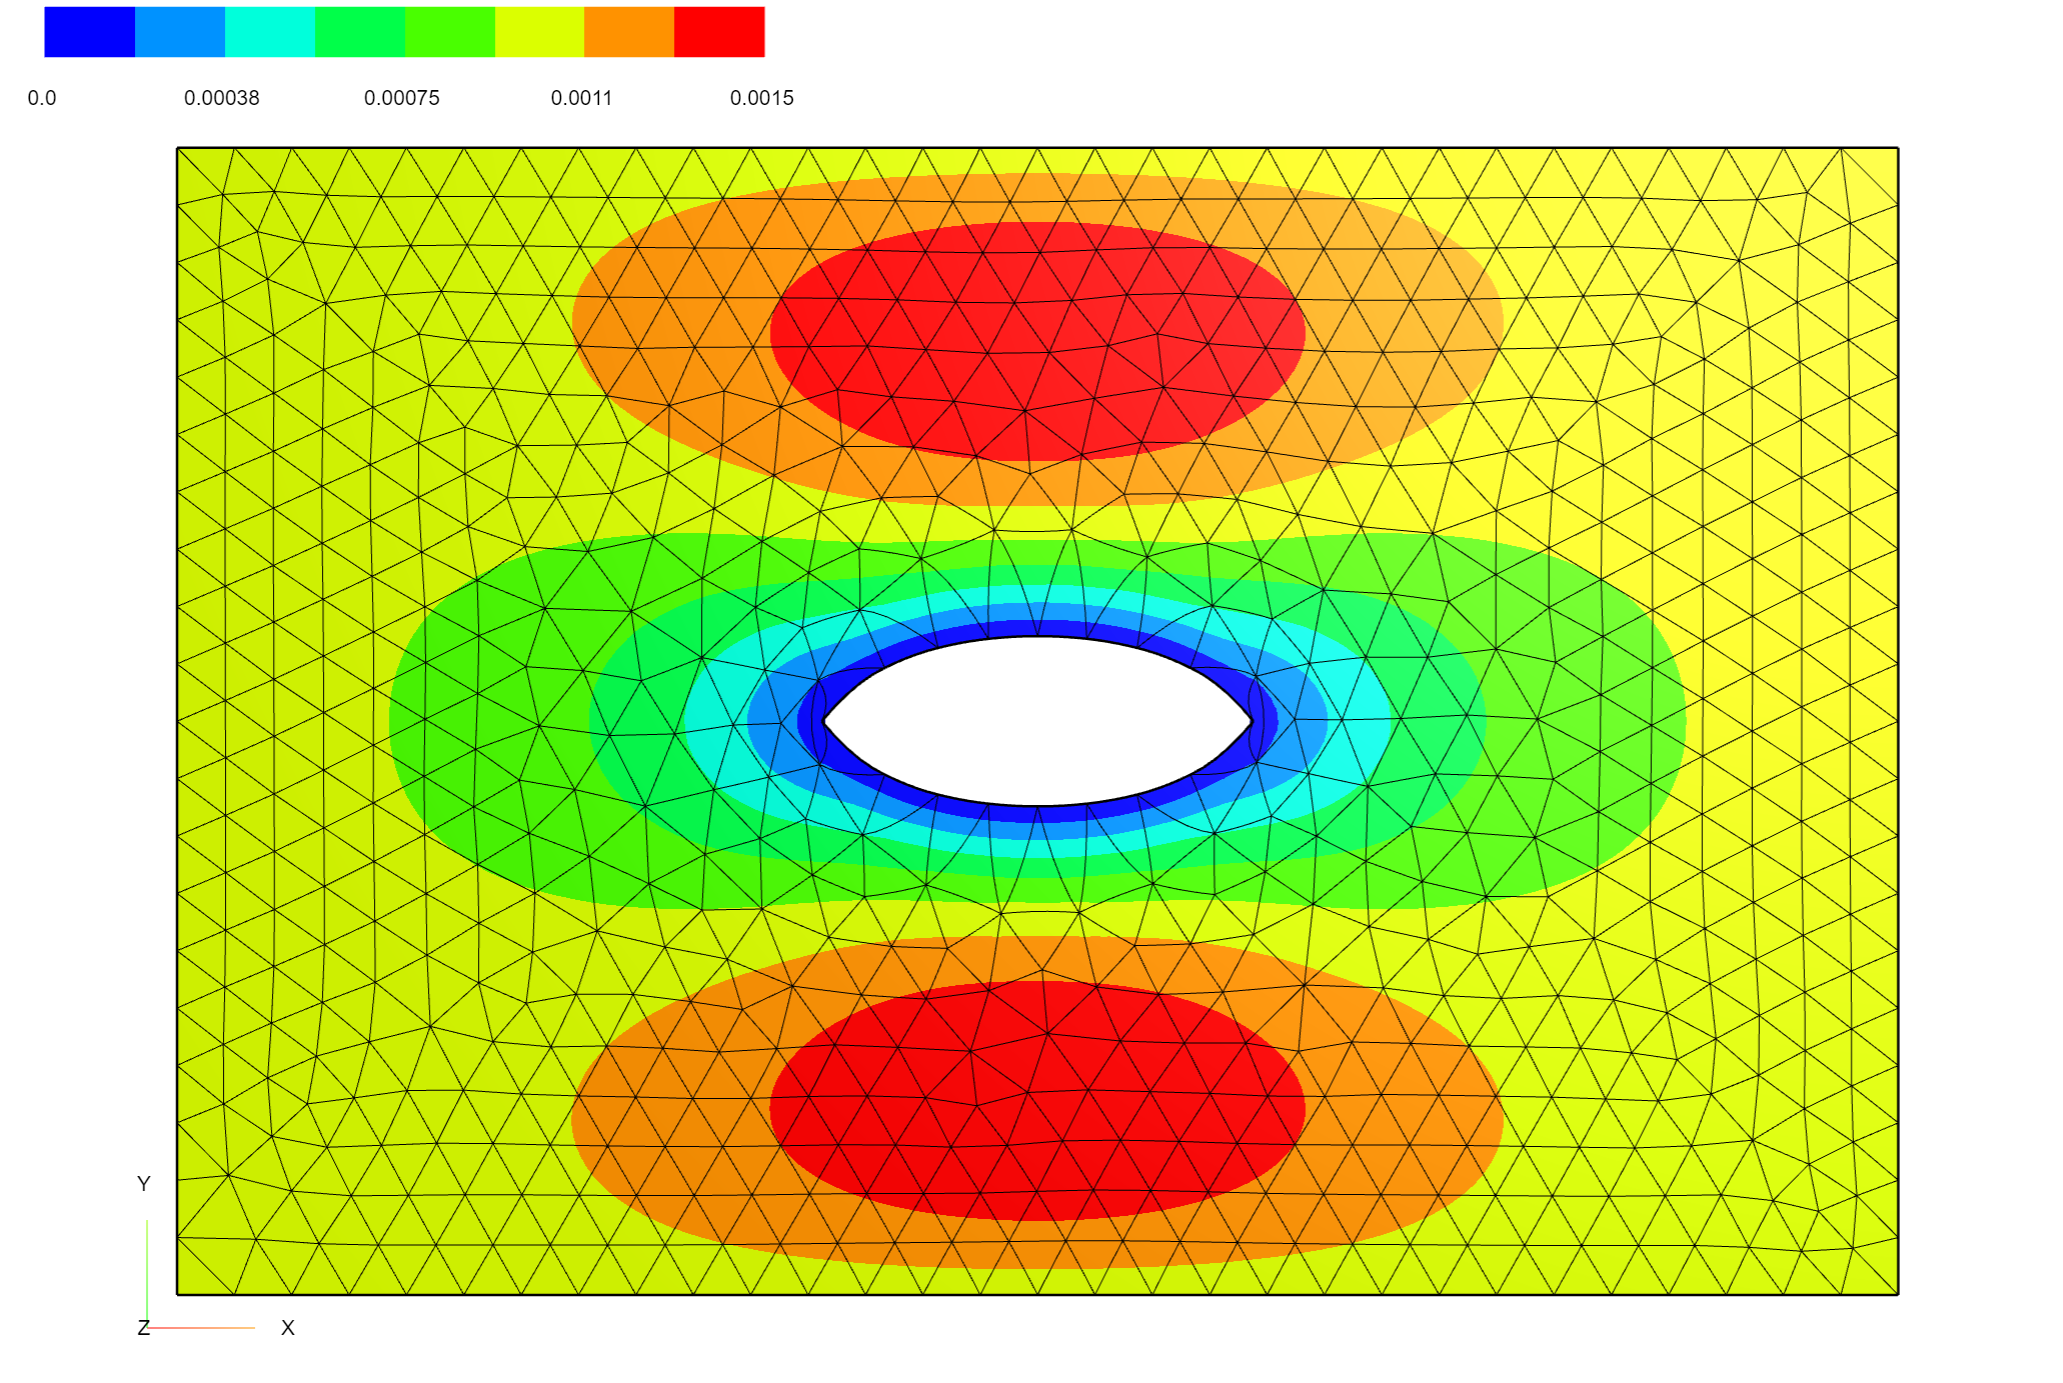
\includegraphics[width=0.8\textwidth]{figures/solution_shape_opt.PNG}
	\caption{Velocity magnitude of Stokes flow after shape optimization}
	\label{shape_opt_plot}
\end{figure}